\documentclass[review]{elsarticle}

\usepackage{lineno,hyperref}
\usepackage{amssymb,amsmath,array}
\usepackage{xcolor}% provides \colorlet
\usepackage{fixme}
\fxsetup{
    status=draft,
    author=,
    layout=inline,
    theme=color
}

\definecolor{fxnote}{rgb}{0.8000,0.0000,0.0000}
% define the background colour:
\colorlet{fxnotebg}{yellow}

% refedine the layout macro:
\makeatletter
\renewcommand*\FXLayoutInline[3]{%
  \@fxdocolon {#3}{%
    \@fxuseface {inline}%
    \colorbox{fx#1bg}{\color {fx#1}\ignorespaces #3\@fxcolon #2}}}
\makeatother

\modulolinenumbers[5]

\journal{Journal of \LaTeX\ Templates}

\newcommand{\IR}{\rm I\!R}

%%%%%%%%%%%%%%%%%%%%%%%
%% Elsevier bibliography styles
%%%%%%%%%%%%%%%%%%%%%%%
%% To change the style, put a % in front of the second line of the current style and
%% remove the % from the second line of the style you would like to use.
%%%%%%%%%%%%%%%%%%%%%%%

%% Numbered
%\bibliographystyle{model1-num-names}

%% Numbered without titles
%\bibliographystyle{model1a-num-names}

%% Harvard
%\bibliographystyle{model2-names.bst}\biboptions{authoryear}

%% Vancouver numbered
%\usepackage{numcompress}\bibliographystyle{model3-num-names}

%% Vancouver name/year
%\usepackage{numcompress}\bibliographystyle{model4-names}\biboptions{authoryear}

%% APA style
%\bibliographystyle{model5-names}\biboptions{authoryear}

%% AMA style
%\usepackage{numcompress}\bibliographystyle{model6-num-names}

%% `Elsevier LaTeX' style
\bibliographystyle{elsarticle-num}
%%%%%%%%%%%%%%%%%%%%%%%

\begin{document}

\begin{frontmatter}

\title{The Conjunctive Disjunctive Graph Node Kernel}
%\tnotetext[mytitlenote]{Fully documented templates are available in the elsarticle package on \href{http://www.ctan.org/tex-archive/macros/latex/contrib/elsarticle}{CTAN}.}

%% Group authors per affiliation:
\author{Dinh Tran Van}
\author{Alessandro Sperduti}
\address{Department of Mathematics, Padova University, Trieste, 63, 35121 Padova, Italy}
\author{Fabrizio Costa}
\address{Department of Computer Science, University of Exeter Exeter EX4 4QF, UK}
%\fntext[myfootnote]{Since 1880.}

%% or include affiliations in footnotes:
%\author[mymainaddress,mysecondaryaddress]{Elsevier Inc}
%\ead[url]{www.elsevier.com}

%\author[mysecondaryaddress]{Global Customer Service\corref{mycorrespondingauthor}}
%\cortext[mycorrespondingauthor]{Corresponding author}
%\ead{support@elsevier.com}

%\address[mymainaddress]{1600 John F Kennedy Boulevard, Philadelphia}
%\address[mysecondaryaddress]{360 Park Avenue South, New York}

\begin{abstract}
Gene-disease associations are inferred on the basis of similarities between the proteins encoded by genes. Biological relationships used to define similarities range from interacting proteins, proteins that participate in pathways and protein expression profiles. Though graph kernel methods have become a prominent approach for association prediction, most solutions are based on a notion of information diffusion that does not capture the specificity of different network parts. Here we propose a graph kernel method that explicitly models the configuration of each gene's context. An empirical evaluation on several biological databases shows that our proposal achieves state-of-the-art results.
\end{abstract}

\begin{keyword}
Graph node kernels, graph decomposition, disease gene prioritization
\end{keyword}
\end{frontmatter}

\linenumbers
\section{Introduction}
Predictive systems for gene-disease associations are often based on a notion of similarity between genes. A common strategy is to encode relations between genes as a network and use graph based techniques to make useful inferences. In the last decades, a number of graph kernel methods have been proposed that directly exploit transitive properties in biological networks. The prototypical method is the Diffusion kernel (DK) \cite{kondor2002diffusion} inspired by the heat diffusion phenomenon. The key idea is to allow a given amount of {\em heat} placed on nodes to {\em diffuse} through the edges. The similarity between two nodes $v_{i}, v_{j}$ is then defined as the amount of heat starting from $v_{i}$ and reaching $v_{j}$ within a given time interval. In DK the heat flow is proportional to the number of paths connecting two nodes, which introduces an undesired bias that penalize peripheral nodes w.r.t. central ones. This problem is tackled by a modified version of DK called Markov exponential diffusion kernel (MED) \cite{chen2014disease} where a Markov matrix replaces the Laplacian matrix.  Another kernel called Markov diffusion kernel (MD) \cite{fouss2006experimental}, exploits instead the notion of {\em diffusion distances}, a measure of similarity between patterns of heat diffusion. The Regularized Laplacian kernel (RL) \cite{chebotarev2006matrix} represents instead a normalized version of the random walk with restart model and defines the node similarity as the number of paths connecting two nodes with different lengths. All these approaches can be applied to dense networks with high degree nodes. A drawback of these approaches is however their relatively low discriminative capacity. This is in part due to the fact that information is processed in an additive and independent fashion which prevents them from accurately modeling the configuration of each gene's context. To address this issue here we propose to employ a {\em decompositional} graph kernel (DGK) \cite{haussler1999convolution} technique in which the similarity function between graphs can be formed by decomposing each graph into subgraphs and by devising a valid local kernel between the subgraphs. To exploit its higher discriminative capacity we first decompose the network in a collection of connected sparse graphs and then we develop a suitable kernel, that we call Conjunctive Disjunctive Node Kernel (CDNK).

\section{Material and methods}
We start from the type of similarity notion computed by decomposition kernels between graph instances and adapt it to express the similarity between nodes in a single network. In this work we use three key ideas: 1) genes are described using their functional profile encoded as a vector of real values, 2) the network is marked to distinguish highly connected components from sparsely connected ones, and 3) we transform the neighborhood of each gene in a sparse high dimensional vector that can be easily processed by standard machine learning techniques such as SVMs.

\textit{Definitions.} 
We represent a problem instance as a graph $G=(V,E)$ where $V$ is the set of nodes and $E$ is the set of links.
We define the \textit{distance} $\mathcal{D}(u,v)$ between two nodes $u$ and $v$, as the number of edges on the shortest path between them. The \textit{neighborhood} of a node $u$ with radius $r$, $N_r(u) = \lbrace v\ |\ d(u,v) \leq r \rbrace$, is the set of nodes at distance no greater than $r$ from $u$. The corresponding \textit{neighborhood subgraph} $\mathcal{N}_{r}^{u}$ is the  subgraph induced by the neighborhood (i.e. considering all the edges with endpoints in $N_r(u)$). The \textit{degree} of a node $u$, $d(u) = |\mathcal{N}_{1}^{u}|$, is the cardinality of its neighborhood. The maximum node degree in the graph $G$ is $d(G)$.


\subsection{Gene Labeling} Gene-disease associations networks typically represent genes as nodes labeled with a gene identifier. Here we take a different approach and use the node labels to encode abstract information about the genes. In this way downstream machine learning algorithms can generalize from similar examples and allow the identification of overlooked but related genes. We experiment with two types of information: 1) topological information and 2) functional information. 

\textit{Topological label.} This information is simply based on the connectivity degree of the gene. The idea is that genes that have the same number of connections are more similar than genes with a different connectivity. The node labeling function $\ell$ assigns the degree for nodes $u$ having degree less than or equal than a user defined threshold $T$ ($T=5$ in our experimental evaluation). However degree values larger than $T$ are subsequently discretized into $k$ levels. Formally, the labeling function is defined as:
\begin{center}
$\ell(u) = \left\{
	\begin{array}{ll}
		d(u),\  & \mbox{if } d(u) \leq T \\
		T+i,\ & \mbox{if } d(u) > T
	\end{array}
\right.$,
\end{center}
where $i = \lceil \frac{d(u)-T}{bin}\rceil$, $bin = \frac{d(G)-T}{\lambda - T}$ and $\lambda$ ($\lambda > T$) is the maximum number of symbols used. The value of $\lambda$ depend on the degree distribution and can be tuned as a hyperparameter of the approach.


\textit{Functional label.} This type of information is based on the \textit{Gene Ontology} \cite{gene2004gene} resource. We use the ontology to construct binary vectors representing a bag-of-words encoding for each gene (i.e. if one of the 26501 GO-terms is associated with the gene). The resulting vectors are then clustered using the k-means algorithm  into a user defined number of classes $K$ (tuned as a hyperparameter of the approach), so that genes with similar description profiles receive the same class identifier as label. 

\textit{Real valued vector information encoding.}
In addition to encoding the functional information as a discrete label we add a richer description by computing the similarity vector w.r.t. to each cluster. In this way we can fully exploit the latent description of the genes in terms of the different functional groups captured by the clustering procedure. Formally, given a vector $v \in \IR^{26501}$ we compute a similarity vector $S(v)= \{s_1, s_2, \ldots s_K\}$ with entries $s_i = \frac{1}{1+d(v,c_i)}$ where $d(v,c_i)$ is the euclidean distance of $v$ from the center of the i$^{th}$ cluster $c_i = \frac{1}{|C_i|}\sum_{x \in C_i} x$ computed as the geometric mean of the elements in the cluster $C_i$.


\subsection{Network Decomposition} 
In gene-disease associations networks it is not uncommon to find nodes with high degrees. Unfortunately these cases cannot be effectively processed by a neighborhood based decomposition kernel since these are based on the notion of exact matches and the probability of finding identical neighborhoods decreases exponentially as the degree increases. This means that in a finite network it quickly becomes impossible to find any match and hence learn or generalize at all. As an alternative, we propose a procedure to ''sparsify'' the network that is observed by the neighborhood kernel. In reality we do not alter the cardinality of the edge set, but rather mark the edges with special attributes that will inform the kernel computation. The result is a procedure that decomposes the network in a linked collection of sparse sub-networks where each node has a reduced connectivity when considering the edges of a specific type. However the other edges are still available to connect the various sub-networks. We distinguish two types of edges: {\em conjunctive} and {\em disjunctive} edges. Nodes linked by conjunctive edges are going to be used jointly to define the notion of context and will be visible to the neighborhood graph kernel. Nodes linked by disjunctive edges are instead used to define features based only on the pairwise co-occurrence of the genes at the endpoints and are processed by our novel kernel.




\textit{Iterative k-core decomposition} \cite{alvarez2005k}: The node set is partitioned in two groups on the basis of the degree of each node w.r.t. a threshold degree $D$, the first part contains all nodes with degree smaller or equal than $D$ and the second part the remaining ones. The node partition is used to induce the ''conjunctive' vs ''disjunctive' notion for the edge partition: edges that have both endpoints in the same part (be it the first or the second) are marked as conjunctive, otherwise they are marked as disjunctive. We apply the k-core decomposition iteratively, where at each iteration we consider only the graph induced by the conjunctive edges. We stop iterating the decomposition after a user defined number of steps. Note that this decomposition does not alter the cardinality of the edge set, it is simply a procedure to mark each edge with the attribute conjunctive or disjunctive.  

\begin{figure}
\centering
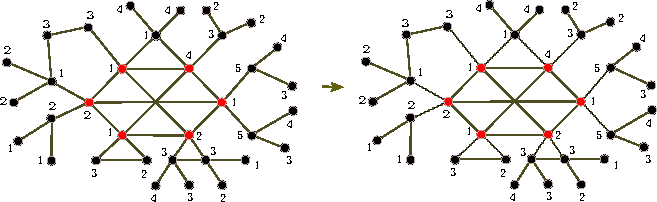
\includegraphics[width=.9\textwidth]{k_core}
\caption{K-core decomposition}
\label{fig:example}
\end{figure}

\textit{Clique decomposition} \cite{tarjan1985decomposition}: To model the notion that nodes in a clique are tightly related, we summarize the whole clique with a new 'representative' node. All the cliques (completely connected subgraphs) with a number of nodes greater than a threshold size $C$ are identified. The endpoints of all edges incident on the clique's nodes are moved to the representative node. Disjunctive edges are introduced to connect each node in the clique to the representative. Finally all edges with both endpoints in the clique are removed.

In our work a network is transformed by applying first the iterative k-core decomposition and then the clique decomposition.

\begin{figure}
\centering
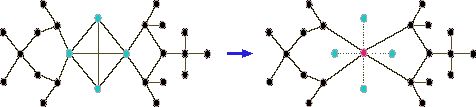
\includegraphics[width=.9\textwidth]{clique}
\caption{Clique decomposition}
\label{fig:example}
\end{figure}

\subsection{Node Graph Kernels} 
We start from the Neighborhood Subgraph Pairwise Distance Kernel (NSPDK) \cite{costa2010fast} and adapt it to express the similarity between nodes in a single network. The key idea in NSPDK is to decompose graphs in small fragments and count how many pairs of fragments are shared between two instances. We introduce two improvements: 1) we partition the features according to the individual node's neighborhood, and 2) we introduce a  distinction between ''disjunctive'' and ''conjunctive'' edges.

\subsubsection{The Neighborhood Subgraph Pairwise Distance Kernel}
The NSPDK is an instance of convolution kernel \cite{haussler1999convolution} where given a graph $G \in \mathcal{G}$ and two rooted graphs $A_u, B_v$, the relation $R_{r,d}(A_u, B_v, G)$ is true {\em iff} $A_u \cong \mathcal{N}_r^u$ is (up to isomorphism $\cong$) a neighborhood subgraph of radius $r$ of $G$ and so is $B_v \cong  \mathcal{N}_r^v$, with roots at distance $\mathcal{D}(u,v)= d$. We denote $R^{-1}$ as the inverse relation that returns all pairs of neighborhoods of radius $r$ at distance $d$ in $G$, $R^{-1}_{r,d}(G) = \lbrace A_u, B_v | R_{r,d}(A_u,B_v,G)=true\rbrace$. The kernel $\kappa_{r,d}$ over $\mathcal{G} \times \mathcal{G}$, counts the number of such fragments in common in two input graphs: 
\begin{center}
$\kappa_{r,d}(G,G^{'}) = 
\!\!\!\!\!\!\!\!\!\!\!\! 
\sum\limits_{\substack{A_u, B_v \ \in \ R_{r,d}^{-1}(G) \\ 
{A'}_{u'}, {B'}_{v'} \ \in \ R_{r,d}^{-1}(G')
}} \!\!\!\!\!\!\!\!\!\!\!\!  { { \textbf{1}_{A_{u} \cong A'_{u'}}} \cdot {
\textbf{1}_{B_{v} \cong B'_{v'}}} }$, 
\end{center} 
\noindent where $\textbf{1}_{A \cong B}$ is the \textit{exact matching function} that returns 1 if $A$ is
isomorphic to $B$ and 0 otherwise.  Finally, the NSPDK is defined as $K(G,G') = \sum\limits_{r}{\sum\limits_{d}{\kappa_{r,d}(G,G')}}$, where for efficiency reasons, the values of $r$ and $d$ are upper bounded to a given maximal $r^*$ and $d^*$, respectively.

\subsubsection{The Conjunctive Disjunctive Node Kernel}
We extend NSPDK and define a node kernel $K(G_u,G_{u'})$ between two copies of the same network $G$ where we distinguish the nodes $u$ and $u'$ respectively. The idea is to define the features of a node $u$ as the subset of NSPDK features that always have the node $u$ as one of the roots. In addition we distinguish between two types of edges, called {\em conjunctive} and {\em disjunctive} edges. When computing distances to induce neighborhood subgraphs, only conjunctive edges are considered. When choosing the
pair of neighborhoods to form a single feature, we additionally consider roots $u$ and $v$ that are not at distance $d$ but such that $u$ is connected to $w$ via a disjunctive edge and such that $w$ is at distance $d$ from $v$. In this way disjunctive edges can still allow an {\em information flow} even if their
endpoints are only considered in a pairwise fashion and not jointly. 

Formally, we define two relations: the \textit{conjunctive relation} $R^{\wedge}_{r,d}(A_u, B_v, G_u)$ identical to the NSPDK relation $R_{r,d}(A_u, B_v, G)$,  and (ii) $\mathcal{D}(u,v)= d$; the \textit{disjunctive relation} $R_{r,d}^{\vee}(A_u, B_v, G_u)$ is true {\em iff} (i)  $A_u \cong \mathcal{N}_r^u$ and $B_v \cong \mathcal{N}_r^u$ are true, (ii) $\exists w$ s.t. $\mathcal{D}(w,v)= d$, and (iii) $(u,w)$ is a disjunctive edge. We define $\kappa_{r,d}$ on the  inverse relations ${R^{\wedge}_{r,d}}^{ -1}$ and ${R^{\vee}_{r,d}}^{ -1}$
\begin{center}
 $\kappa_{r,d}(G_u,G_{u'}) = \!\!\!\!\!\!\!\!\!\!\!\!
 \sum\limits_{\substack {A_u,{B}_{v} \in {R_{r,d}^{\wedge}}^{ -1}(G_u) \\ A'_{u'},{B'}_{v'} \in {R_{r,d}^{\wedge}}^{ -1}(G_{u'}) }} \!\!\!\!\!\!\!\!\!\!\!\!
  { \textbf{1}_{A_u \cong A'_{u'}} \cdot { \textbf{1}_{B_{v} \cong B'_{v'}}}}
+ \!\!\!\!\!\!\!\!\!\!\!\!
 \sum\limits_{\substack {A_u,{B}_{v} \in {R_{r,d}^{\vee}}^{ -1}(G_u) \\
  A'_{u'},{B'}_{v'} \in \ {R_{r,d}^{\vee}}^{ -1}(G_{u'}) }} \!\!\!\!\!\!\!\!\!\!\!\!
  { \textbf{1}_{A_u \cong A'_{u'}} \cdot { \textbf{1}_{B_{v} \cong B'_{v'}}}}
  $.
\end{center}
The CDNK is finally defined as $K(G_u,G_v) = \sum\limits_{r}{\sum\limits_{d}{\kappa_{r,d}(G_u,G_v)}}$, where once again for efficiency reasons, the values of $r$ and $d$ are upper bounded to a given maximal $r^*$ and $d^*$.


\subsection{Real valued node information}
In order to process real vectors we do a convolution of the vector with the node sparse vector.




\section{Experimental}
We perform an empirical evaluation of the predictive performance of several kernel based methods on two of the databases used in \cite{chen2014disease}.

\textbf{BioGPS:} A gene co-expression network is constructed from BioGPS dataset, which contains 79 tissues, measured with the Affymetrix U133A array. Edges are inserted when the pairwise Pearson correlation coefficient (PCC) between genes is larger than 0.5.

\textbf{Pathways:} Pathway information is retrieved from KEGG, Reactome, PharmGKB and the Pathway Interaction Database. If a couple of proteins co-participate in any pathway, the two corresponding genes are linked.  

To evaluate the performance of graph node kernels we analyze the {\em gene prioritization}, i.e. given a set of genes known to be associated to a given disease, gene prioritization is the task to rank the candidate genes based on their probabilities to be related to that disease. Similar to the evaluation process used in \cite{chen2014disease}, we choose 12 diseases \cite{goh2007human} with at least 30 confirmed genes. For each disease, we construct a positive set $\mathcal{P}$ with all confirmed disease genes, and a negative set $\mathcal{N}$ which contains random genes associated at least to one disease class which is not related to the class that is defining the positive set. In \cite{chen2014disease} the ratio between the dataset sizes is chosen as $\vert \mathcal{N} \vert = \frac{1}{2} \vert \mathcal{P} \vert$. The predictive performance of each method is evaluated via a leave-one-out cross validation: one gene is kept out in turn and the rest are used to train an SVM model. We compute a decision score $q_i$ for the test gene $g_i$ as the top percentage value of score $s_i$ among all candidate gene scores. We collect all decision scores for every gene in the training set to form a global decision score list on which we compute the AUC ROC.

\textbf{Model Selection:}
The hyper parameters of the various methods are set using a k-fold on a dataset set that is then never used in the predictive performance estimate. We try the values for diffusion parameter in DK and MED in $\lbrace 10^{-3}, 10^{-3}, 10^{-2}, 10^{-1} \rbrace$, time steps in MD in $\lbrace 1, 10, 100 \rbrace$ and RL parameter in $\lbrace 1, 4, 7 \rbrace$. For CDNK, we try for the degree threshold values in $\lbrace 10,\ 15,\ 20 \rbrace$, clique size threshold in $\lbrace 4,\ 5 \rbrace$, maximum radius in $\lbrace 1,\ 2 \rbrace$, maximum distance in $\lbrace 2,\ 3,\ 4 \rbrace$. Finally, the regularization trade off parameter $C$ for the SVM is searched in $\lbrace 10^{-5},  \ 10^{-4}, \ 10^{-3},\ 10^{-2},\ 10^{-1}, 1,\ 10,\ 10^2 \rbrace$.
\section{Results and discussion}
Table \ref{table_biogps} and \ref{table_pathways} show the AUC performance of the models trained by using different graph node kernels on 11 gene-disease association problems using the BioGPS and Pathways datasets to materialize the gene relation network. We note that CDNK ranks first in 7 out of 11 cases using  both networks. CDNK is the top performant kernel also when considering the average AUC ROC and the average rank with 73.3/2.0, 76.5/1.8, with a difference w.r.t. the second best of 5.5$\%$ and 1$\%$ on BioGPS and Pathways, respectively. MED and RL show similar and moderate results with small gap between them. DK and MD exhibit modest performance on average and  are ranked last in many cases: 7 times out of 11 for MD in BioGPS and 10 out of 11 for DK in Pathways. Low performance cases include networks that have high {\em average} node degree which is likely to yield very sparse and fragmented network decompositions.
%======================================================
\begin{table}
\centering
\setlength{\tabcolsep}{1mm}
\begin{tabular}{|c|c|c|c|c|c|c|c|c|}
\hline
         & \multicolumn{8}{c|}{\textbf{BioGPS}}\\
 \hline
Disease & DK & MD & MED & RL & CDNK1 & CDNK2 & CDNK3 & CDNK4\\

 \hline
1 & 51.9/8 & 57.4/7 & 59.0/6 & 59.2/5 & 65.1/4 & 69.5/2 & 69.3/3 & \textbf{70.3/1} \\
2 & 81.7/5 & 78.5/6 & 75.2/7 & 75.0/8 & 88.3/2 & \textbf{88.8/1} & 85.1/4 & 86.8/3 \\
3 & 64.3/7 & 59.6/8 & 71.6/3 & 71.8/2 & 65.5/5 & \textbf{72.5/1} & 64.7/6 & 66.4/4 \\
4 & 65.3/7 & 58.2/8 & 67.8/6 & 67.8/5 & 71.9/4 & \textbf{78.7/1} & 73.9/3 & 77.0/2 \\
5 & 64.0/8 & 64.1/7 & 66.5/5 & 66.2/6 & 75.9/4 & 76.2/3 & 76.9/2 & \textbf{77.4/1} \\
6 & 74.6/5 & 70.2/8 & 71.0/7 & 71.2/6 & 79.3/2 & \textbf{83.7/1} & 76.7/4 & 79.0/3 \\
7 & 73.0/5 & 66.7/8 & 75.4/3 & 75.6/2 & 68.8/6 & 73.9/4 & 67.3/7 & \textbf{76.9/1} \\
8 & 74.4/8 & 76.8/3 & 76.2/5 & 76.4/4 & 74.7/7 & \textbf{77.7/1} & 76.0/6 & 76.8/2 \\
9 & 71.5/2 & 65.6/8 & 67.7/5 & 69.9/3 & 66.8/7 & \textbf{71.7/1} & 67.1/6 & 68.1/4 \\
10 & 54.0/6 & 50.3/8 & 56.1/5 & 51.1/7 & 77.6/4 & \textbf{82.7/1} & 80.5/2 & 80.0/3 \\
11 & 58.2/7 & 51.3/8 & 59.3/6 & 59.3/5 & 71.8/4 & \textbf{80.2/1} & 75.3/3 & 77.1/2 \\
\hline
$\overline{AUC}$ & 66.6 & 63.5 & 67.8 & 67.6 & 73.2 & \textbf{77.8} & 73.9 & 76.0 \\
$\overline{Rank}$ & 	6.18 & 7.18 & 5.27 & 4.82 & 4.45 & \textbf{1.55} & 4.18 & 2.36 \\
 \hline 
\end{tabular}
\caption{\textit {Predictive performance on 11 gene-disease associations in percentage using network induced by the BioGPS. Best results are in bold. We report the AUC ROC and the rank for each kernel method in which CDNK1 uses ontology for discrete labels, CDNK2 uses ontology for both discrete and continous labels, CDNK3 uses node degree for discrete labels and CDNK4 uses degree and ontology for both discrete and continous labels, respectively.}}
\label{table_biogps}
\end{table}
%==================================================
\begin{table}
%\vspace*{-5pt}
\centering
\setlength{\tabcolsep}{1mm}
\begin{tabular}{|c|c|c|c|c|c|c|c|c|}
\hline
         & \multicolumn{8}{c|}{\textbf{Pathways}} \\
 \hline
Disease & DK & MD & MED & RL & CDNK1 & CDNK2 & CDNK3 & CDNK4 \\

 \hline
1 & 74.7/8 & 76.4/7 & 78.7/6 & 78.8/5 & 80.2/3 & \textbf{82.4/1} & 80.6/2 & 79.4/4 \\
2 & 55.1/8 & 64.9/7 & 76.6/6 & 76.6/5 & 81.1/2 & 80.3/3 & 79.8/4 & \textbf{82.2/1} \\
3 & 55.0/8 & 62.7/7 & 64.1/5 & 65.6/4 & 67.1/3 & 63.6/6 & 68.5/2 & \textbf{71.5/1} \\
4 & 54.3/8 & 65.2/7 & \textbf{73.7/1} & 73.7/2 & 66.1/5 & 68.1/3 & 67.5/4 & 65.6/6 \\
5 & 52.9/8 & 55.7/7 & 62.7/5 & 62.7/6 & 68.3/2 & \textbf{69.6/1} & 66.3/4 & 66.8/3 \\
6 & 83.4/8 & 92.7/7 & 96.5/2 & \textbf{96.5/1} & 93.0/6 & 94.1/5 & 94.4/4 & 95.5/3 \\
7 & 84.5/8 & 88.3/7 & 89.4/3 & 89.5/2 & 88.5/6 & 88.5/5 & 88.7/4 & \textbf{90.5/1} \\
8 & 53.7/8 & 65.6/7 & 72.0/6 & 72.3/5 & 72.5/3 & 72.5/2 & 72.3/4 & \textbf{76.5/1} \\
9 & 52.5/8 & 64.9/5 & 64.2/7 & 64.2/6 & \textbf{81.3/1} & 81.0/2 & 79.6/3 & 78.8/4 \\
10 & 68.8/6 & 65.4/8 & 74.4/5 & 74.4/4 & 66.9/7 & 76.8/2 & 76.1/3 & \textbf{79.5/1} \\
11 & 53.7/8 & 69.2/7 & 74.6/5 & 74.1/6 & 77.0/2 & \textbf{78.7/1} & 75.4/4 & 77.0/3 \\
\hline
$\overline{AUC}$ & 62.6 & 70.1 & 75.2 & 75.3 & 76.5 & 77.8 & 77.2 & \textbf{78.5} \\
$\overline{Rank}$ & 7.82 & 6.91 & 4.64 & 4.18 & 3.64 & 2.82 & 3.45 & \textbf{2.55} \\
 \hline 
\end{tabular}
\caption{\textit {Predictive performance on 11 gene-disease associations in percentage using network induced by the Pathways. Best results are in bold. We report the AUC ROC and the rank for each kernel method in which CDNK1 uses ontology for discrete labels, CDNK2 uses ontology for both discrete and continous labels, CDNK3 uses node degree for discrete labels and CDNK4 uses degree and ontology for discrete and continous labels, respectively.}}
\label{table_pathways}
\end{table}

\section{Conclusions}
We have shown how decomposing a network in a set of connected sparse graphs allows us to take advantage of the discriminative power of CDNK, a novel decomposition kernel, to achieve state-of-the-art results. In future work we will investigate how to 1) decompose networks in a data driven way and 2) extend the CDNK approach to gene-disease association problems exploiting multiple heterogeneous information sources in a joint way.
%\section{The Elsevier article class}
%
%\paragraph{Installation} If the document class \emph{elsarticle} is not available on your computer, you can download and install the system package \emph{texlive-publishers} (Linux) or install the \LaTeX\ package \emph{elsarticle} using the package manager of your \TeX\ installation, which is typically \TeX\ Live or Mik\TeX.
%
%\paragraph{Usage} Once the package is properly installed, you can use the document class \emph{elsarticle} to create a manuscript. Please make sure that your manuscript follows the guidelines in the Guide for Authors of the relevant journal. It is not necessary to typeset your manuscript in exactly the same way as an article, unless you are submitting to a camera-ready copy (CRC) journal.
%
%\paragraph{Functionality} The Elsevier article class is based on the standard article class and supports almost all of the functionality of that class. In addition, it features commands and options to format the
%\begin{itemize}
%\item document style
%\item baselineskip
%\item front matter
%\item keywords and MSC codes
%\item theorems, definitions and proofs
%\item lables of enumerations
%\item citation style and labeling.
%\end{itemize}
%
%\section{Front matter}
%
%The author names and affiliations could be formatted in two ways:
%\begin{enumerate}[(1)]
%\item Group the authors per affiliation.
%\item Use footnotes to indicate the affiliations.
%\end{enumerate}
%See the front matter of this document for examples. You are recommended to conform your choice to the journal you are submitting to.
%
%\section{Bibliography styles}
%
%There are various bibliography styles available. You can select the style of your choice in the preamble of this document. These styles are Elsevier styles based on standard styles like Harvard and Vancouver. Please use Bib\TeX\ to generate your bibliography and include DOIs whenever available.
%
%Here are two sample references: \cite{Feynman1963118,Dirac1953888}.

\section*{References}

\bibliography{mybibfile}

\end{document}